\documentclass[../../FisicaTeorica.tex]{subfiles}

\begin{document}
Chiaramente, due osservabili $A$ e $B$ possono essere (banalmente) compatibili se uno è una funzione dell'altro, $B=f(A)$. Si dicono allora \textbf{dipendenti}, e le misure di una \textit{determinano} le misure dell'altra.
In particolare si avrà $\sigma(B)=\sigma(f(A))=f(\sigma(A))$. Se ciò non succede,\ $A$ e $B$ si dicono \textbf{indipendenti}.\\
Notiamo che la dipendenza di osservabili compatibili si può verificare sperimentalmente (possiamo misurare entrambe le osservabili e vedere se il valore di una coincide con $f$ calcolata nel valore dell'altra).\\
\begin{dfn}
Un insieme $\mathcal{C}$ di osservabili compatibili indipendenti si dice \textbf{completo} se è massimale, ossia se non esiste alcun insieme di osservabili compatibili indipendenti che lo contenga propriamente (non si può trovare insiemi strettamente \q{più grandi}). Quindi $\mathcal{C}$ è completo se una qualunque misura di I specie di un'ulteriore osservabile indipendente che non si trova in $\mathcal{C}$ comporta necessariamente l'aumento delle fluttuazioni di almeno una delle osservabili di $\mathcal{C}$ (ossia eseguire una misura di un qualsiasi osservabile non compresa tra quelle in $\mathcal{C}$ \textit{disturba} quelle delle osservabili in $\mathcal{C}$).
\end{dfn}
Per le osservabili a spettro discreto, il risultato di una misura di I specie è l'individuazione del sottospazio di $\hs$ corrispondente all'autovalore trovato (quello \textit{compatibile} con la misura ottenuta).\\
Ci aspettiamo allora che, una volta misurate tutte le osservabili in $\mathcal{C}$, si abbia un'informazione \textit{massimale} sul sistema, ossia che la misura di tutte le $\mathcal{C}$ proietti il sistema su uno \textbf{stato puro}.

\begin{thm}
Sia $\mathcal{C}=\{A_1, \dots, A_n\}$\marginpar{ICOC (a spettro discreto)} un insieme di osservabili compatibili indipendenti a spettro discreto. Allora $\mathcal{C}$ è \textbf{completo} se e solo se le osservabili $A_1, \dots, A_n$ hanno un insieme completo (cioè una base tale da verificare la completezza di Dirac) di autovettori comuni \textbf{senza degenerazione}.\\
In altre parole:
\[
\dim \hs_{(a_1,\dots,a_n)}=1\quad \forall (a_1,\dots,a_n)\in \sigma(A_1,\dots,A_n)
\]
\end{thm} 
\textbf{Dim}. Partiamo dimostrando che \textit{non degenere} $\Rightarrow$ \textit{completo}.         
Consideriamo un'osservabile $B$ compatibile con tutte le osservabili in $\mathcal{C}$, e verifichiamo che, se la base di autovettori comuni non ha degenerazione, $B$ deve essere per forza \textbf{dipendente}, ossia funzione delle osservabili in $\mathcal{C}$.\\
Indichiamo con $\{(\ket{(a_1,\dots, a_n)}\}$ gli autovettori comuni di $\mathcal{C}$, dove $(a_1, \dots, a_n)\in\sigma(\mathcal{C})$ sono gli autovalori comuni delle osservabili $A_1, \dots, A_n \in \mathcal{C}$ (e in generale, come visto precedentemente, $\sigma(\mathcal{C})\neq \sigma(A_1)\times \dots \times \sigma(A_n)$).\\
Per ipotesi di compatibilità, tali autovettori costituiscono una base completa. Se, in più, non vi è degenerazione, la completezza di Dirac si scrive come:
\begin{equation}
\sum_{(a_1 \dots a_n)\in \sigma(\mathcal{C})} \ket{(a_1, \dots, a_n)}\bra{(a_1, \dots, a_n)}=\bb{I}
\label{eqn:completezza_base_comune}
\end{equation}
Poiché $B$ è compatibile con $\mathcal{C}$, ogni $\ket{(a_1, \dots, a_n)}$ deve essere anche autovettore di $B$ e quindi anche della famiglia spettrale $P^B(\lambda)$  di $B$ per il teorema (\ref{thm:compatibility}).\\
Vale allora l'equazione agli autovalori per $P^B(\lambda)$:
\begin{equation}
P^B(\lambda)\ket{(a_1, \dots, a_n)}=f_\lambda(a_1, \dots, a_n) \ket{(a_1, \dots, a_n)}
\label{eqn:proiettori_base_comune}
\end{equation}
dove gli \textit{autovalori} sono dati da una qualche funzione $f_\lambda(a_1,\dots, a_n)$, che è iniettiva per la non-degenerazione (cambiare uno degli $a_i$ significa considerare un altro autovettore, che deve quindi avere un altro autovalore poiché tutti gli autospazi hanno dimensione $1$. Ma allora $f$ manda punti diversi in punti diversi).\\
Allora combinando (\ref{eqn:completezza_base_comune}) con (\ref{eqn:proiettori_base_comune}) si ha:
\begin{align*}
P^B(\lambda)\bb{I} &= P^B(\lambda)=\sum_{(a_1, \dots, a_n)\in \sigma(\mathcal{C})} f_\lambda(a_1, \dots, a_n)\ket{(a_1, \dots, a_n)}\bra{(a_1, \dots, a_n)}\\ 
&\equiv f_\lambda(A_1,\dots, A_n)
\end{align*} %[DOMANDA] Perché questo ragionamento non funzione se c'è degenerazione? f non è più iniettiva, e allora?
dove si è usata la definizione di rappresentazione spettrale di una funzione delle osservabili.\\
Quindi $B$ è una funzione di $\mathcal{C}$ individuata da:
\[
B=\int_\bb{R} \lambda\,dP^B(\lambda) =\int_\bb{R} \lambda\,df_\lambda(A_1,\dots, A_n)
\] 
ed è pertanto dipendente da $\mathcal{C}$, quindi $\mathcal{C}$ è completo.\\

Viceversa, dimostriamo che se vi è \textbf{degenerazione} $>1$ allora $\mathcal{C}$ \textbf{non} è \textbf{completo}.\\
Supponiamo che per qualche autovalore $(a_1, \dots, a_n) \in \sigma(\mathcal{C})$ l'autospazio $\hs_{(a_1,\dots,a_n)}$ abbia dimensione $d(a_1, \dots, a_n)>1$ (ossia vi è degenerazione).\\
Allora dato un operatore $B$ autoaggiunto non banale in $\hs_{(a_1,\dots, a_n)}$ (ossia una qualsiasi matrice hermitiana in questo autospazio che non sia nulla o multiplo dell'identità), lo estendiamo all'identità sul complemento di $\hs_{(a_1,\dots, a_n)}$ in $\hs$ (cioè lo estendiamo ad un operatore $\tilde{B}$ definito su tutto $\hs$ che è pari a $B$ sull'autospazio $\hs_{(a_1, \dots, a_n)}$, e agisce come l'identità su tutto il resto).\\
Nella base comune di $\mathcal{C}$, la forma matriciale di $B$ è allora del tipo:
\[
\tilde{B}=
\begin{pmatrix}
1 & \cdots & \cdots & \cdots & \cdots & \cdots & 0\\
\vdots &\ddots & 0&  &  & & \vdots\\
\vdots & 0 & 1 & 0 & & &\vdots \\
\vdots & \vdots& 0 & \boxed{B} & 0 & & \vdots \\
\vdots & & & 0 & 1 & 0 & \vdots\\
\vdots & & &\ & 0 & \ddots & 0\\
0& \cdots & \cdots& \cdots & \cdots & 0 & 1
\end{pmatrix}
\]
Dove il blocco centrale ha dimensione pari alla degenerazione $d(a_1, \dots, a_n)$, e quindi è certamente più grande di un $1\times 1$.\\
Tale rappresentazione matriciale mostra che $B$ manda vettori dell'autospazio $\hs_{(a_1,\dots,a_n)}$ in vettori che rimangono al suo interno, e quindi \textit{non disturba} le misure di tutti gli altri operatori, e infatti commuta\footnote{Pià precisamente, basta seguire passi analoghi alla dimostrazione del teorema di compatibilità. In particolare, $B$ è per ipotesi autoaggiunto, e quindi ammette una base su $\hs_{(a_1,\dots,a_n)}$ che diagonalizza il \textit{blocco centrale}. Ma allora ha una base di autovettori comune a tutte le $\mathcal{C}$, e quindi è compatibile con esse.} con $A_1, \dots, A_n$.\\
Tuttavia, se misuriamo $A_1,\dots,A_n$ e otteniamo come risultato $(a_1,\dots,a_n)$ lo stato del sistema sarà una combinazione lineare degli autostati di $B$ (data la degenerazione), e scegliendo opportunamente $B$ in modo che abbia più di un autovalore, il risultato di una seguente misura di $B$ non è determinato.\\
Abbiamo allora trovato un operatore $\tilde{B}$ che è compatibile con tutti i $\mathcal{C}$ e non dipende funzionalmente da essi: perciò $\mathcal{C}$ non è completo.
\begin{flushright}
$\square$
\end{flushright}

\begin{oss}
Poiché una misura su un Insieme Completo di Osservabili Compatibili (ICOC) $\mathcal{C}$ a spettro discreto identifica uno spazio $1-$dimensionale in $\hs$, tale misura può essere usata per preparare uno stato puro.
\end{oss}
\begin{oss}
Sotto opportune condizioni sugli spazi nucleari $\phi_{A_1,\dots,A_n}$ comuni a $\mathcal{C}$ (che generalizzano la nozione di \textit{autospazio comune}), il teorema precedente si estende ad un ICOC a spettro arbitrario, includendo gli autovettori generalizzati (cioè possiamo usarlo anche per \textit{spettri continui}).
\end{oss}
Questo consente di dare una definizione precisa di \textbf{rappresentazione}\marginpar{Rappresentazioni}\index{Rappresentazione} $\mathcal{C}$.\\
Partiamo scrivendo la \textit{completezza generalizzata}\footnote{La produttoria è data dal fatto che stiamo considerando l'applicazione simultanea di più osservabili. Per esempio, se $A\ket{\psi}=a\ket{\psi}$ e $B\ket{\psi}=b\ket{\psi}$, con $A$ e $B$ compatibili si ha $AB\ket{\psi}=ab\ket{\psi}$. Si noti inoltre l'assenza di sommatorie sugli indici di degenerazione, dato che per un ICOC gli autovettori sono \textit{nondegeneri} per ipotesi.} per un ICOC $\mathcal{C}$:
\[
\prod_{i=1}^n \left(\sum_{a_i \in \sigma_P(A_i)} + \int_{\sigma_C(A_i)} da_i\right) \ket{(a_1,\dots,a_n)}\bra{(a_1,\dots,a_n)}=\bb{I}
\]
ove $\ket{(a_1, \dots, a_n)}$ sono autovettori (generalizzati) comuni di $\mathcal{C}$ \textbf{nondegeneri}. Perciò ogni vettore $\ket{(a_1, \dots, a_n)}$ è univocamente individuato dai valori $(a_1, \dots, a_n)$ e ogni $\ket{\psi}\in \hs$ si può scrivere:
\[
\ket{\psi}=\prod_{i=1}^n \left(\sum_{a_i\in \sigma_P(A_i)} + \int_{\sigma_C(A_i)}da_i \right) \ket{(a_1, \dots, a_n)}\braket{(a_1, \dots, a_n)|\psi}
\]
Quindi i coefficienti $\{\braket{(a_1, \dots, a_n)|\psi}=\psi(a_1, \dots, a_n)\}$, con $(a_1, \dots, a_n)\in \sigma(\mathcal{C})$, identificano univocamente lo stato $\ket{\psi}$ e vengono detti definire lo stato in \textbf{rappresentazione }$\mathcal{C}$.\\
Per esempio, supponiamo $\mathcal{C}=\{\vec{X}\}$, allora sappiamo che:
\[
\braket{\vec{x}|\psi}=\psi(\vec{x})
\]
Se invece $\mathcal{C}=\{\vec{P}\}$, allora:
\[
\braket{\vec{p}|\psi}=\tilde{\psi}(\vec{p})
\]
Per una particella in $\bb{R}^3$ potremmo scegliere $\mathcal{C}=\{X,P_y, Z\}$, mentre in $\bb{R}$ si può avere $\mathcal{C}=\{H, \mathcal{P}\}$, dato che se $[H,\mathcal{P}]=0$ \textit{rimuove} la degenerazione degli autovalori di $H$.

\begin{dfn}
Un insieme di osservabili $\mathcal{I}$ (non compatibili!) si dice \textbf{irriducibile} se ogni osservabile che commuta con tutti gli elementi di $\mathcal{I}$ è un multiplo dell'identità $\bb{I}$ (ossia il risultato della sua misura è  \textbf{indipendente dello stato} - es. come nel caso dell'osservabile che misura la carica elettrica dell'elettrone).\\
Ciò significa che misurare tutte le osservabili in $\mathcal{I}$ non può ridurre il sistema ad uno stato di massima informazione (puro).%Controllare se l'intuizione è giusta 9[TO DO]
\end{dfn}
\begin{oss}
Per una particella quantistica elementare \textit{con analogo classico}\footnote{Ossia senza proprietà unicamente quantistiche, come lo \textit{spin}} $\{\vec{X},\vec{P}\,\}$ è un insieme irriducibile.\\ %Cosa si intende per analogo classico? [DOMANDA]
Infatti sia $A$ un'osservabile che commuta con $\vec{X}$, poiché $\mathcal{C}=\{\vec{X}\}$ è un ICOC, necessariamente $A=f(\vec{X})$. Ma se $A$ commuta anche con $\vec{P}$, vuol dire che (usando la rappresentazione in $\vec{x}$):
\begin{align*}
0&=[\vec{P}, \underbrace{f(\vec{X})}_{A}]\psi(\vec{X})=
\vec{P}(f(\vec{X})\psi(\vec{X}))-f(\vec{X})\vec{P}(\psi(\vec{X}))=\\
&=-i\hbar \vec{\nabla}(f(x)\psi(x))+i\hbar f(\vec{x})\vec{\nabla}\psi(\vec{x}) = -i\hbar(\vec{\nabla}f)(\vec{x})\psi(\vec{x})=0 \quad \forall \psi
\end{align*}
Ma allora $f$ è una costante:
\[
\vec{\nabla}f(\vec{x})=0=f(\vec{x})=\text{cost.}
\]
\end{oss}

\section{Esercizio 2}
Una particella di massa $m$ in 1D è immersa nel potenziale (buca infinita):
\[
V(x)=\begin{cases}
0 & |x|<\frac{a}{2}\\
+\infty & \text{altrove}
\end{cases}
\]
Sia $\mathcal{E}=\frac{2\pi^2\hbar^2}{ma^2}$ l'energia dello stato a $t=-t_0$ ($t_0>0$).\marginpar{Richieste dell'esercizio}
\begin{enumerate}
\item All'istante $t=0$ una misura (ideale di I specie) rivela la presenza della particella nella parte destra della buca. Determinare la funzione d'onda dopo la misura.
%[IMMAGINE] Disegnetto della buca con oscurata la parte sinistra (dove non è stata trovata la particella)
\item All'istante $t_0$ si esegue una misura\footnote{Che, quando non specificato diversamente, è da intendersi come ideale di prima specie.}, determinare la probabilità di trovare un'energia più alta di quelle a $t=t_0$.
\item Determinare la probabilità di trovare il valore $+1$ eseguendo una misura di \textit{parità} $\mathcal{P}$ a $t=t_0$
\item Determinare $(\Delta X)_{\psi}(\Delta P)_\psi$ per tutti gli stati stazionari $\psi$\ del sistema.
\item Si dica se $P$ (con condizioni periodiche) e $H$ sono compatibili.
\item Si determini la probabilità di trovare la particella nella metà sinistra della buca per $0<t<t_0$.
\end{enumerate}

\subsection{Soluzione}
\begin{enumerate}
\item Dalla soluzione del potenziale della buca infinita (CFR sezione \ref{sec:buca_infinita_1D}) sappiamo che gli autovalori di $H$ sono:
\begin{equation}
\bm{\mathcal{E}_n} = \frac{\hbar^2}{2m}\frac{n^2 \pi^2}{a^2}
\label{eqn:autoval_buca_infinita}
\end{equation}
e le rispettive autofunzioni sono:
\[
\bm{\varphi_n}(x)=\begin{cases}
\sqrt{\frac{2}{a}}\cos\left(\frac{n\pi x}{a}\right) & n \in \bb{N} \text{ dispari }\\
\sqrt{\frac{2}{a}}\sin\left(\frac{n\pi x}{a}\right) & n\in \bb{N} \text{ pari}
\end{cases}
\]
\begin{figure}[H]
\centering
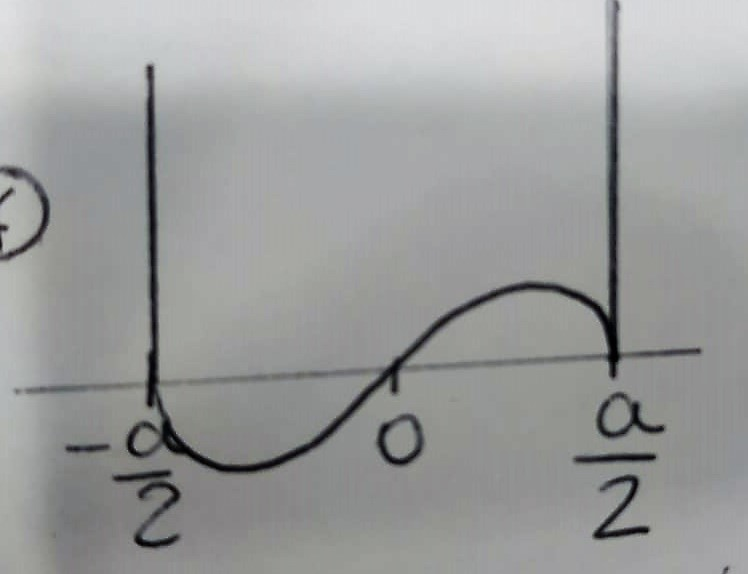
\includegraphics[scale=0.4]{Immagini/15_11/img2.jpeg}
\caption{$\psi$ iniziale}
\end{figure}
Ricordiamo che gli autovalori $\mathcal{E}_n$ \textbf{non hanno degenerazione}: ogni $\mathcal{E}_n$ si ottiene per due valori, $n$ e $-n$, che però definiscono \textit{lo stesso stato}. Basta infatti sostituirli nelle $\varphi_n$: nel caso dispari non cambia nulla, e in quello pari si ottiene un cambio di segno, ossia uno sfasamento che non modifica l'autostato.\\ 
Notiamo che l'energia iniziale assegnata $\mathcal{E}=\mathcal{E}_2$ (chiaramente il valore assegnato \textbf{deve} essere uno di quelli possibili, dato che non ogni valore è possibile come in \MC).\\
Lo stato $\ket{\psi_0}$ a $t=-t_0$ è allora un \textbf{autostato} di $H$ (per la precisione $\ket{\varphi_2}$, autofunzione di autovalore $\mathcal{E}_2$). Si tratta allora di uno \textbf{stato stazionario}, ossia di uno stato che rimane inalterato fino a che il sistema resta isolato, ossia fino a quando non si effettua una misura.\\
Matematicante, gli \textit{stati stazionari}\marginpar{Stati stazionari}\index{Stato!stazionario} sono le soluzioni dell'equazione di Schr\"odinger stazionaria, che in effetti è proprio l'equazione agli autovalori di $H$: $H\ket{\psi}=\mathcal{E}\ket{\psi}$.\\
Se esaminiamo l'evoluzione di $\ket{\psi_0}$ applicando direttamente la formula (\ref{eqn:evoluzione_temporale_totale}), otteniamo infatti un conto \textit{semplice}:
\[
\ket{\psi(t)}=e^{-\frac{i}{\hbar}t\mathcal{E}_n} \ket{\mathcal{E}_2}\underbrace{\braket{\mathcal{E}_2|\psi_0}}_{\braket{\varphi_2|\varphi_2}=1} = e^{-\frac{i}{\hbar}\mathcal{E}_2 t} \ket{\psi_0}
\]
Dato che tutti gli altri termini della sommatoria sono nulli, essendo $\ket{\psi_0}=\ket{\varphi_2}=\ket{\mathcal{E}_2}$.\\
Il conto appena fatto mostra come l'evoluzione temporale della $\ket{\psi_0}$ sia un'\textit{oscillazione di fase}. Se esaminiamo la parte reale (o immaginaria) della $\ket{\psi(t)}$ osserviamo infatti un'\textit{onda stazionaria}.
\\
\begin{figure}[H]
\centering
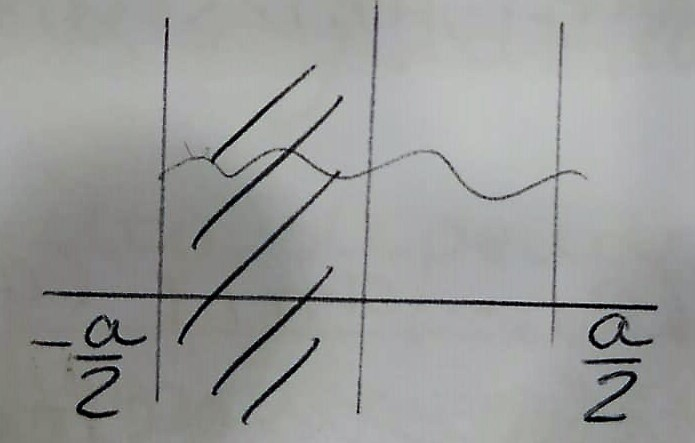
\includegraphics[scale=0.4]{Immagini/15_11/img1.jpeg}
\caption{Effetto della misura}
\end{figure}

\begin{figure}[H]
\centering
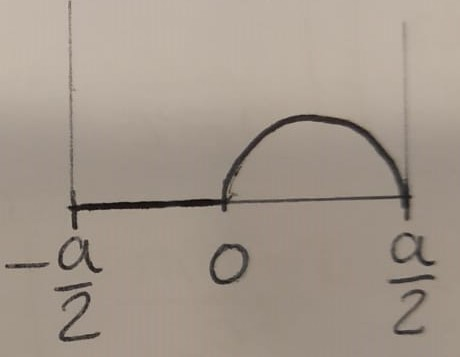
\includegraphics[scale=0.6]{Immagini/15_11/img3.jpeg}
\caption{$\psi$ dopo la misura}
\end{figure}
Calcolando per $t=0$ giungiamo allora a:
\[
\psi(x,t=0)=e^{-\frac{i}{\hbar}t_0\mathcal{E}_2} \psi(x,-t_0)
\]
Ma la $\psi(x,-t_0)$ di partenza è definita a meno di una fase, e possiamo sceglierla opportunamente in modo che l'esponenziale generato dall'evoluzione temporale scompaia.
Giungiamo allora a:
\[
\psi(x,0^-)=\sqrt{\frac{2}{a}} \sin\left(\frac{2\pi x}{a}\right)
\]
A $t=0$ l'atto di misura proietta (assioma di von Neumann) la funzione d'onda sugli autostati compatibili con la misura osservata:
\[
\psi(x,0^+) = P^X\left(\left[0,\frac{a}{2}\right]\right)\psi(x,0^-)=A\begin{cases}
\sqrt{\frac{2}{a}}\sin\left(\frac{2\pi x}{a}\right) & 0 <x<\frac{a}{2}\\
0 & -\frac{a}{2}<x<0
\end{cases}
\]
Dove $A$ è la nuova costante di normalizzazione per $\psi(x,0^+)$.\\
Poiché $\psi(x,0)$ era già un autostato, la parte di essa che fa parte del \q{dominio compatibile con la misura}, ossia $[0,+a/2]$, viene \textit{proiettata su se stessa}, e quindi non cambia. Tutto il resto viene invece portato a $0$.\\
Normalizziamo per trovare $A$:
\begin{align*}
1&\overset{!}{=}\int_{-\frac{a}{2}}^{+\frac{a}{2}} dx\,|\psi(x,0^+)|^2 = |A|^2 \int_0^{+\frac{a}{2}} \frac{2}{a}\sin^2\left(\frac{2\pi x}{a}\right)=\\
&=|A|^2 \int_0^{+\frac{a}{2}} \frac{2}{a}\frac{1}{2}\left(1-\cos\left(\frac{4\pi x}{a}\right)\right) dx =\\
&=\frac{|A|^2}{a} \frac{1}{2}\left[x-\frac{a}{4\pi}\sin\left(\frac{4\pi x}{a}\right)\right]_0^{+\frac{a}{2}} =|A|^2 \frac{1}{a} \frac{a}{2} = \frac{|A|^2}{2}=1\Rightarrow A=\sqrt{2}
\end{align*}
Perciò:
\[
\psi(x,0^+)=\begin{cases}
\frac{2}{\sqrt{a}}\sin\left(\frac{2\pi x}{a}\right) & 0<x<+\frac{a}{2}\\
0 & -\frac{a}{2}<x<0
\end{cases}
\]
Notiamo che $\psi(x,0^+)$ \textbf{non} è più un autostato di $H$.\\
\item Per i calcoli di probabilità è necessaria la funzione d'onda al tempo $t_0>0$. Per determinare $\psi(x,t)$ per $t>0$ (fino a $t_0$) dobbiamo \textbf{espandere} $\psi(x,0^+)$ negli \textbf{autostati} $\varphi_n(x)$ di $H$:
\[
\psi(x,0^+)=\sum_{n=1}^{\infty} \underbrace{(\varphi_n, \psi(x,0^+))}_{c_n}\varphi_n(x)
\]
Da cui la formula (\ref{eqn:evoluzione_temporale_totale}) conduce a:
\[
\psi(x,t)=\sum_{n=1}^\infty c_n e^{-\frac{i}{\hbar}\mathcal{E}_n t}\varphi_n(x)
\]
Determiniamo quindi i $c_n$. Per $n$ pari, ed essendo $\varphi_n$ a valori reali:
\[
c_n = \int_{\bm{0}}^{+\frac{a}{2}} \underbrace{\sqrt{\frac{2}{a}} \sin\left(\frac{n\pi x}{a}\right)}_{\varphi_n^*=\varphi_n} \underbrace{\frac{2}{\sqrt{a}}\sin\left(\frac{2\pi x}{a}\right)}_{\psi(x,0^+)}\,dx
\]
Applicando le formule di Werner:
\[
\sin(\alpha)\sin(\beta)=\frac{1}{2}\left(\cos(\alpha-\beta)-\cos(\alpha+\beta)\right)
\]
Si ha che:
\[
c_n = \frac{\cancel{2}\sqrt{2}}{a}\int_0^{+\frac{a}{2}} \frac{1}{\cancel{2}} \left[\cos \frac{(n-2)\pi x}{a}-\cos\frac{(n+2)\pi x}{a}\right]
\]
Per $n\neq 2$ si ottiene (ricordando che $n$ pari):
\[
\frac{\sqrt{2}}{a}\left[\frac{a}{(n-2)\pi}\sin\frac{(n-2)\pi x}{a}\Big|_0^{+\frac{a}{2}} - \frac{a}{(n+2)\pi}\sin\frac{(n+2)\pi x}{a}\Big|_0^{+\frac{a}{2}}\right] = 0
\]
Per $n=2$ la funzione integranda è $\sin^2$, e perciò:
\begin{align*}
c_2&=\frac{2\sqrt{2}}{a}\int_0^{+\frac{a}{2}}\sin^2\left(\frac{2\pi x}{a}\right)dx =\\
&= \frac{\cancel{2} \sqrt{2}}{a \, \cancel{2}}\left[
x-\frac{a}{4\pi}\sin\left(\frac{4\pi x}{a}\right)\right]_0^{+\frac{a}{2}} =
\frac{\sqrt{2}}{\cancel{a}}\frac{\cancel{a}}{2}=\frac{1}{\sqrt{2}}
\end{align*}

Per $n$ dispari, analogamente:\lesson{22}{16/11/2018}
\[
c_n=\int_0^{+\frac{a}{2}} \sqrt{\frac{2}{a}}\cos\left(\frac{n\pi x}{a}\right)\frac{2}{\sqrt{a}}\sin\left(\frac{2\pi x}{a}\right)\,dx
\]
Applicando le formule di Werner:
\[
\sin(\alpha) \cos (\beta) = \frac{1}{2}\left(\sin(\alpha+\beta)+\sin(\alpha-\beta)\right)
\]
si giunge a:
\begin{align*}
c_n &= \int_0^{\frac{a}{2}}\frac{2\sqrt{2}}{a}\frac{1}{2}\left[\sin\frac{(2+n)\pi x}{a}+\sin\frac{(2-n)n x}{a}\right]dx =\\
&= \frac{\sqrt{2}}{\bcancel{a}}\left[ \frac{\bcancel{a}}{(2+n)\pi}\left(-\cos \frac{(n+2)\pi x}{a}\right)\Big|_{0}^{\frac{a}{2}}+\frac{\bcancel{a}}{(2-n)\pi}\left(-\cos\frac{(2-n)\pi x}{a}\right)\Big|_{0}^{\frac{a}{2}} \right] =\\
&=\sqrt{2}\left[\frac{1}{(2+n)\pi} + \frac{1}{(2-n)\pi}\right]=\sqrt{2}\frac{4}{4-n^2}\frac{1}{\pi}
\end{align*}
Riepilogando, i valori di $c_n=(\varphi_n, \psi(x,0^+))$ sono dati da:
\begin{align*}
\text{$n$ pari} && \begin{cases}
c_n = 0 \quad n \neq 2\\
c_2 = \frac{1}{\sqrt{2}}
\end{cases}\\
\text{$n$ dispari} && c_n=\sqrt{2}\frac{4}{4-n^2}\frac{1}{\pi}
\end{align*}
Possiamo finalmente calcolare la probabilità che la nuova funzione d'onda abbia a $t_0$ energia più alta di $\mathcal{E}_2$. Ciò è equivalente al problema (più semplice) di calcolare la probabilità che $\ket{\psi}$ \textbf{non} abbia energia pari a $\mathcal{E}_1$ o a $\mathcal{E}_2$. Applicando allora la formula (\ref{eqn:probability_discreta}) (che è già stata vista proprio nel caso della buca infinita in (\ref{eqn:calcolo_prob})):
\begin{align*}
P^H_{\psi(t)}(\mathcal{E}>\mathcal{E}_2)&=1-W^H_{\psi(t)}(\mathcal{E}_1)-W^H_{\psi(t)}(\mathcal{E}_2)\\
W^H_{\psi(t)}(\mathcal{E}_n) &= |(\psi(t),\varphi_n)|^2 = |(\psi(0^+),\varphi_n)|^2 = |c_n|^2
\end{align*}
dato che $\psi(t)=U(t)\psi(0^+)$, e $U(t)$ è unitario, cioè aggiunge solo una fase $\exp\left(-\frac{i}{\hbar}\mathcal{E}_n t\right)$ alla $\psi(0^+)$, senza modificare il modulo.\\
Svolgendo allora i conti:
\[
P_{\psi(t)}^H(\mathcal{E}>\mathcal{E}_2)=1-|c_1|^2-|c_2|^2=1-\left|\sqrt{2}\left(\frac{1}{\pi}+\frac{1}{3\pi}\right)
\right|^2 -\frac{1}{2} \sim 0.14
\]
\item Calcoliamo ora la probabilità che la parità applicata a $\psi(t_0)$ dia $+1$, ossia $W_{\psi(t_0)}^\mathcal{P}(+1)$. Sappiamo che la parità agisce come:
\[
\mathcal{P}\psi(x,t_0)=\psi(-x,t_0)
\]
Per calcolare $W_{\psi_{t_0}}(+1)$ dobbiamo costruire il proiettore $P^\mathcal{P}(\{+1\})$ che proietta un generico stato $\ket{\psi}$ nell'autospazio di $\mathcal{P}$ di autovalore $+1$. Una base di questo autospazio è per esempio data dalle $\varphi_n$ con $n$ dispari (i $\cos$, che sono pari), e quindi $+1$ è autovalore a degenerazione $\infty$.\\
Infatti, dato che $[H,\mathcal{P}]=0$, $H$ e $\mathcal{P}$ ammettono una base di autovettori comuni. In particolare, una base comune per $H$ e l'autospazio di $\mathcal{P}$ corrispondente all'autovalore $+1$ è data dai $\ket{n}$ con $n$ dispari, la cui rappresentazione in $x$ è:
\[
\braket{x|n}=\cos\left(\frac{n\pi x}{a}\right)
\]
Il relativo proiettore $P^{\mathcal{P}}(\{+1\})$ si ottiene quindi per somma infinita dei proiettori su tali autostati:
\[
P^{\mathcal{P}}(\{+1\}) =\sum_{n \text{ dispari}} \ket{n}\bra{n}
\]
Analogamente, l'autospazio di $\mathcal{P}$ di autovalore $-1$ è generato dai $\ket{n}$ con $n$ pari e:
\[
\braket{x|n}=\sin\left(\frac{n\pi x}{a}\right); \qquad P^{\mathcal{P}}(\{-1\})=\sum_{n \text{ pari}}\ket{n}\bra{n}
\]
Tuttavia, possiamo evitare di calcolare una somma infinita per trovare il proiettore, notando che $\mathcal{P}^2=\bb{I}$, da cui $(1+\mathcal{P})/2$ è un proiettore. Infatti:
\[
\left(\frac{1+\mathcal{P}}{2}\right) \left(\frac{1+\mathcal{P}}{2}\right)=\frac{1}{4}+\frac{1}{2}\mathcal{P}+\frac{1}{4}\mathcal{P}^2=\frac{1}{4}+\frac{1}{2}\mathcal{P}+\frac{1}{4}=\frac{1+\mathcal{P}}{2}
\]
E tale operatore agisce come:
\[
\frac{1+\mathcal{P}}{2}\psi(x)=\frac{\psi(x)+\psi(-x)}{2} = \begin{cases}
\psi(x) & \text{se $\psi(x)$ è pari}\\
0 & \text{se $\psi(x)$ è dispari}
\end{cases}
\]
Quindi $(1+\mathcal{P})/2$ è il proiettore che proietta nell'autospazio $+1$ di $\mathcal{P}$ che volevamo. La probabilità cercata è allora: %Aggiungere qualche passaggio intermedio
\begin{align*}
W_{\psi(t)}^\mathcal{P}(+1)&=\left(\psi(t),\frac{\bb{I}+\mathcal{P}}{2}\psi(t)\right)\underset{(a)}{=}\\
&=\left(
\sum_n c_n \exp\left(-\frac{i}{\hbar}\mathcal{E}_n t\right) \varphi_n, \left(\frac{\bb{I}+\mathcal{P}}{2}\right)\underbrace{
\sum_m c_m \exp\left(-\frac{i}{\hbar}\mathcal{E}_m t\right) \varphi_m}_{m \text{ dispari}} \right) \underset{(b)}{=} \\
&=\sum_{n, m \text{ dispari}} c_n^* c_m \exp\left(-\frac{i}{\hbar}(\mathcal{E}_m-\mathcal{E}_n)t\right)\underbrace{(\varphi_n, \varphi_m)}_{\delta_{nm}}=\sum_{n \text{ dispari}}|c_n|^2
\end{align*}
dove in (a) si sono sviluppate le $\psi(t)$ sulla base degli autostati di $H$ come da formula (\ref{eqn:evoluzione_temporale_totale}), e in (b) si è ristretta la somma ai soli indici negativi, dato che, nel secondo membro del prodotto scalare, all'applicazione del proiettore \q{sopravvivono} solo le $\varphi_m$ pari, che sono quelle dove l'indice $m$ è dispari.\\
Di nuovo, non serve calcolare la somma infinita per $W_{\psi(t)}^{\mathcal{P}}(+1)$, poiché sappiamo che, per il caso opposto di $W_{\psi(t)}^\mathcal{P}(-1)$, la somma è costituita da un solo termine (in quanto solo $c_2 \neq 0$). Basterà allora calcolare la probabilità che l'operatore parità non dia $-1$:
\[
W_{\psi(t)}^\mathcal{P}(+1)=1-W_{\psi(t)}^\mathcal{P}(-1)=1-|c_2|^2=1-\frac{1}{2}=\frac{1}{2}
\]
\item Gli stati stazionari sono gli autostati dell'Hamiltoniana $H$, ossia le $\varphi_n$. Dobbiamo allora calcolare $(\Delta X)_{\varphi_n}(\Delta P)_{\varphi_n}$.\\
\textbf{Nota}: Nei prossimi passaggi semplificheremo la notazione, abbreviando il valor medio di $O$ su $\varphi_n$ con $\langle O \rangle_{\varphi_n} \equiv \langle O \rangle_n$ (omettendo la $\varphi$).\\
Partiamo calcolando $(\Delta X)_n$ per $n$ dispari:
\begin{align*}
(\Delta X)_{\varphi_n}&\equiv(\Delta X)_{n} = \sqrt{\langle X^2\rangle_n - \langle X\rangle^2_n}\\
\underbrace{\langle X^2\rangle_n}_{n \text{ dispari}} &= \braket{\varphi_n|X^2 \varphi_n} = \braket{\varphi_n|x^2 \varphi_n}=\int_{-\frac{a}{2}}^{+\frac{a}{2}}\varphi_n^*(x)x^2 \varphi_n(x) \underset{\substack{\varphi_n(x)\in\bb{R}\\\Rightarrow \varphi_n(x)^*=\varphi_n(x)}}{=} \\
&= \int_{-\frac{a}{2}}^{+\frac{a}{2}}\sqrt{\frac{2}{a}}\left(\cos\frac{n\pi x}{a}\right)x^2 \sqrt{\frac{2}{a}}\left(\cos\frac{n\pi x}{a}\right)dx =\\
&=\int_{-\frac{a}{2}}^{\frac{a}{2}} x^2 \cos^2 \frac{n\pi x}{a} dx = \frac{\bcancel{2}}{a} \int_{-\frac{a}{2}}^{\frac{a}{2}} \frac{x^2}{\bcancel{2}}\left(1+ \cos\frac{2n\pi x}{a}\right)dx =\\
&=\frac{1}{a}\frac{x^3}{3}\Big|_{-\frac{a}{2}}^{+\frac{a}{2}}+\frac{1}{a}\frac{a}{2\pi n}\int_{-\frac{a}{2}}^{+\frac{a}{2}} x^2 \frac{d}{dx}\sin\frac{2n\pi x}{a}dx \underset{\text{per parti}}{=}\\
&=\frac{a^2}{12}+\frac{1}{2\pi n} x^2 \bcancel{\sin\frac{(2n\pi x)}{a}\Big|_{-\frac{a}{2}}^{+\frac{a}{2}}} - \frac{1}{2\pi n}\int_{-\frac{a}{2}}^{+\frac{a}{2}} 2x \sin \frac{2n\pi x}{a} dx=\\
&=\frac{a^2}{12} - \frac{a}{2(\pi n)^2} x \cos\frac{2\pi n x}{a}\Big|_{-\frac{a}{2}}^{\frac{a}{2}} + \frac{a}{2(n\pi)^2}\int_{-\frac{a}{2}}^{\frac{a}{2}} \cos \frac{2n\pi x}{a} dx=\\
&=\frac{a^2}{12}+\frac{a}{2(n\pi)^2}\frac{a}{2}2(-1)^n + \frac{a}{2(\pi n)^2}\frac{a}{2\pi n}\bcancel{\sin\frac{2\pi n x}{a}\Big|_{-\frac{a}{2}}^{\frac{a}{2}}} =\\
&=a^2 \left(\frac{1}{12}-\frac{1}{2(n\pi)^2}\right)\\ \langle X\rangle_n &= \int_{-\frac{a}{2}}^{+\frac{a}{2}}\sqrt{\frac{2}{a}}\left( \cos \frac{n\pi x}{a}\right)x\, \sqrt{\frac{2}{a}}\left( \cos \frac{n\pi x}{a}\right)dx =\\
&=\frac{1}{a}\left( \left[\frac{x^2}{2}\right]^{+\frac{a}{2}}_{-\frac{a}{2}} + \int_{-\frac{a}{2}}^{+\frac{a}{2}} x\cos\left(\frac{2n\pi x}{a}\right) dx\right) \underset{(a)}{=} 0
\end{align*}
Dato che in (a) stiamo integrando una funzione \textit{dispari} su un dominio simmetrico attorno a $0$.\\
Perciò ($n$ dispari):
\begin{align*}
(\Delta X)_n &= a\sqrt{\frac{1}{12}-\frac{1}{2(n\pi)^2}}
\end{align*}
Calcoliamo ora la fluttuazione del momento:
\[
(\Delta P)_n = \sqrt{\langle P^2 \rangle_n - \langle P \rangle^2_n}
\]
$\langle P^2\rangle_n$ lo possiamo ricavare direttamente ricordando che $P^2$ è funzione di $H$, e sappiamo già i valor medi di $H$ nei suoi autostati: $\langle H \rangle_n = \mathcal{E}_n$. Ricordando la (\ref{eqn:autoval_buca_infinita}) otteniamo:
\[
\langle P^2\rangle_n = \langle 2mH\rangle_n = 2m \frac{\hbar^2}{2m}\frac{\pi^2 n^2}{a^2}=\frac{\hbar^2 \pi^2 n^2}{a^2}
\]
Ricordiamo però che il dominio di $P$ su un insieme compatto (come l'intervallo $[-a/2,+a/2]$ che stiamo considerando) richiede, oltre all'integrabilità in modulo quadro e alla regolarità, anche delle \textit{condizioni periodiche} (altrimenti $P$ non è autoaggiunto).\\
Perciò, quando calcoliamo il valor medio:
\[
\langle P \rangle_n =\ \braket{\varphi_n |P\varphi_n}
\]
dobbiamo verificare che le $\varphi_n \in D(P)$.\\
Le \textit{condizioni periodiche} necessarie perché una $\psi$ regolare e modulo quadro integrabile sia in $D(P)$ sono:
\[
\psi\left(-\frac{a}{2}\right)=\psi\left(\frac{a}{2}\right)
\]
E si verifica immediatamente che le $\varphi_n$ le rispettano:
\[
\varphi_n\left(-\frac{a}{2}\right)=0=\varphi_n\left(\frac{a}{2}\right)
\]
E allora $\varphi_n \in D(P)$ e possiamo calcolare il valor medio:
\begin{align*}
\langle P \rangle_n &= \int_{-\frac{a}{2}}^{+\frac{a}{2}}\sqrt{\frac{2}{a}}\cos\left(\frac{n\pi x}{a}\right) \left(-i\hbar\frac{d}{dx}\right) \sqrt{\frac{2}{a}}\cos\left(\frac{n\pi x}{a}\right)= 
\\
&=\frac{2}{a}i\hbar \frac{n\pi}{a} \int_{-\frac{a}{2}}^{+\frac{a}{2}} \cos\left(\frac{n\pi x}{a}\right) \sin\left(\frac{n\pi x}{a}\right) = 0
\end{align*}
(dato che stiamo integrando una funzione dispari su un dominio centrato in $0$). Perciò: 
\[
(\Delta P)_n = \frac{\hbar \pi n}{a}
\]
E quindi il prodotto delle incertezze diviene:
\[
(\Delta X)_n(\Delta P)_n =a \sqrt{\frac{1}{12}-\frac{1}{2(n\pi)^2}}\frac{\hbar \pi n}{a}=\hbar \pi n \sqrt{\frac{1}{12}-\frac{1}{2(\pi n)^2}} \neq 0 \quad \forall n \text{ dispari}
\]

Notiamo che per $n$ pari il calcolo di $(\Delta P)_n$ non cambia. Per il calcolo $(\Delta X)_n$, invece, notiamo che si ha sempre $\langle X\rangle_n = 0$ per un conto analogo a prima. Allo stesso modo si vede che $\langle X^2 \rangle_n$ assume lo stesso valore, ma lo ricalcoleremo illustrando qualche \textit{trucco} per velocizzare il processo. Per $n$ pari:
\begin{align*}
\langle X^2\rangle_n &= \braket{\varphi_n | x^2 \varphi_n} = \int_{-\frac{a}{2}}^{+\frac{a}{2}} \frac{2}{a}\sin^2 \left(\frac{n\pi x}{a}\right) x^2\,dx=\\
&= \frac{\bcancel{2}}{a}\frac{1}{\bcancel{2}} \int_{-\frac{a}{2}}^{+\frac{a}{2}} x^2 \left(1-\cos\left(\frac{2n\pi x}{a}\right)\right)dx =\\
&= \frac{1}{a}\left(\left[\frac{x^3}{3}\right]_{-\frac{a}{2}}^{\frac{a}{2}}- \int_{-\frac{a}{2}}^{+\frac{a}{2}} x^2 \cos\left(\frac{2n\pi x}{a}\right) dx\right)
\end{align*}
Come è noto, quando si valuta una primitiva su un dominio simmetrico, se la primitiva è pari allora il risultato è nullo, e se è dispari basta valutarla all'estremo positivo e moltiplicare per $2$:
\[
f(x) \text{ pari} \Rightarrow [f(x)]_{-a}^{+a}=0; \qquad f(x) \text{ dispari}\Rightarrow [f(x)]_{-a}^{+a}=2f(a)
\]
Perciò immediatamente:
\[
\left[\frac{x^3}{3}\right]_{-\frac{a}{2}}^{+\frac{a}{2}}=\frac{2}{3}\left(\frac{a}{2}\right)^3=\frac{a^3}{12}
\]
Il secondo integrale, invece, lo svolgiamo tramite \textit{metodo tabulare}\footnote{Si tratta di uno schema per ripetere velocemente multiple integrazioni per parti senza confondersi. Più informazioni qui: \url{bit.ly/2BpkiwQ}}, ossia derivando e integrando ripetutamente e scrivendo i risultati in colonne:
\[
\begin{array}{c|c}
x^2 & \cos\left(\frac{2n\pi x}{a}\right)\\ \hline 
-2x & \frac{a}{2n\pi}\sin\left(\frac{2n\pi x}{a}\right)\\
2 & -\left(\frac{a}{2n\pi}\right)^2\cos\left(\frac{2n\pi x}{a}\right)\\
0 & -\left(\frac{a}{2n\pi}\right)^3 \sin\left(\frac{2n\pi x}{a}\right)
\end{array}
\]
Da cui si ottiene immediatamente:
\begin{align*}
&\int_{-\frac{a}{2}}^{+\frac{a}{2}} x^2 \cos\left(\frac{2n\pi x}{a}\right)\,dx = \\
&= \left[
x^2 \sin\left(\frac{2n\pi x}{a}\right)\frac{a}{2n\pi} + 2x \cos\left(\frac{2n\pi x}{a}\right)\left(\frac{a}{2n\pi}\right)^2-2\sin\left(\frac{2n\pi x}{a}\right)\left(\frac{a}{2n\pi}\right)^3
 \right]_{-\frac{a}{2}}^{+\frac{a}{2}}
\end{align*}
Notiamo che tutti e tre gli addendi sono funzioni dispari, e quindi basta calcolarle in $+a/2$. Valutando $\sin$ e $\cos$
\[
\left(\frac{2n\pi x}{a}\right)\Big|_{x=\frac{a}{2}} = n\pi \Rightarrow \sin(n\pi)=0;\quad \underbrace{\cos(n\pi)}_{n \text{ pari}}=+1
\]
Perciò primo e terzo termine si annullano, e basta valutare il secondo in $a/2$ e raddoppiare per simmetria:
\[
\int_{-\frac{a}{2}}^{+\frac{a}{2}}x^2 \cos\left(\frac{2n\pi x}{a}\right) = \bcancel{2} \cdot \bcancel{2} \cdot \frac{a}{2} \cdot (+1) \frac{a^2}{\bcancel{4}(n\pi)^2} = \frac{a^3}{2(n\pi)^2}
\]
Mettendo tutto insieme si giunge a:
\[
\langle X^2 \rangle_n = a^2\left(\frac{1}{12}-\frac{1}{2(n\pi)^2} \right)
\]
e perciò $(\Delta X)_n$ ha lo stesso valore sia per $n$ pari che per $n$ dispari, così come $(\Delta P)_n$. Allora, in generale:
\[
(\Delta P)_n(\Delta X)_n = \hbar \pi n \sqrt{\frac{1}{12}-\frac{1}{2(\pi n)^2}} \neq 0 \quad \forall n
\]
\item $H$ e $P$ sono compatibili?\\
Se $H$ e $P$ sono compatibili, ammettono una base di autovettori comuni. Come ricordato all'inizio, gli autostati $\varphi_n$ di $H$ sono non degeneri, e quindi sono già una base ortonormale. Ma allora, per la compatibilità, i $\varphi_n$ dovrebbero essere anche autostati di $P$: ciò non è possibile perché $(\Delta P)_n \neq 0$ come abbiamo appena visto al punto precedente, e perciò $H$ e $P$ \textbf{non} sono compatibili.\\
\textbf{Nota} che $P$ e $P^2$ sono compatibili, $P^2$ e $H$ sono compatibili, ma $P$ e $H$ non lo sono! In generale:
\[
[P^2, H]=0, \> [P,P^2]=0 \not\Rightarrow [P,H]=0
\]
La compatibilità è una questione delicata da valutare attentamente sempre \textit{mediante} la definizione, dato che potrebbero sorgere problemi di dominio (per esempio $P$ e $H$ sono compatibili nel caso libero, ma non in questo caso \textit{compatto}).
\item Vogliamo ora trovare la probabilità di trovare la particella nella metà sinistra della buca per tempi $t$ tra $0$ e $t_0$, ossia, per l'\textit{assioma  della probabilità}, $P_{\psi(t)}^X \left(\left[-\frac{a}{2},0\right]\right)$, con $0<t<t_0$.
Essendo $\psi(t)$ già normalizzata, ossia $\norm{\psi(t)}^2=1$, e ricordando la famiglia spettrale dell'operatore $X$ vista in (\ref{eqn:famiglia_spettrale_x}), si giunge a: 
\begin{align*}
P_{\psi(t)}^X \left(\left[-\frac{a}{2},0\right]\right) &= \left(\psi(t), P^X\left(\left[-\frac{a}{2},0\right]\right)\psi(t)\right)=\\
&=\left(\psi(t), \left[P^X(0)-P^X\left(-\frac{a}{2}\right)\right]\psi(t)\right)=\\
&= \int_{\bb{R}}\psi^*(t)\left (H\left(-x\right)-H\left(-\frac{a}{2}-x\right)\right)\psi(t)=\\
&=\int_{-\frac{a}{2}}^{0} |\psi(x,t)|^2 dx=\\
&= \int_{-\frac{a}{2}}^0 \sum_n c_n^* \sum_m c_m \exp\left(\frac{i}{\hbar}(\mathcal{E}_n-\mathcal{E}_m)t\right)\varphi_n^*(x)\varphi_m(x)dx=\\
&=\sum_{n,m}c_n^* c_m \gamma_{nm}\exp\left(\frac{i}{\hbar}(\mathcal{E}_n-\mathcal{E}_m)t\right) \quad \gamma_{nm}\equiv \int_{-\frac{a}{2}}^0 \varphi_n^*(x) \varphi_n(x) dx 
\end{align*}
Per cui, la probabilità che una misura di $X$ trovi la particella in un dato intervallo è semplicemente l'integrale del modulo quadro della funzione d'onda (in rappresentazione in $x$) in quell'intervallo.\\
Per $m,n$ dispari, per $m\neq n$ applichiamo le formule di Werner e otteniamo un risultato nullo (le primitive dei $\cos$ sono $\sin$ che si annullano in $0$ e $-a/2$), mentre per $m=n$ si ha l'integrale del $\cos^2$, che si scompone con bisezione:
\begin{align*}
\gamma_{mn}&=\frac{2}{a}\int_{-\frac{a}{2}}^0 \cos\left( \frac{n\pi x}{a}\right)\cos\left( \frac{m\pi x}{a}\right)dx=\frac{1}{a}\int_{-\frac{a}{2}}^{0} \left[
\cos\frac{(n+m)\pi x}{a}+ \cos\frac{(n-m)\pi x}{a}
\right]dx=\\
&=\begin{cases}
0 & n\neq m\\
\displaystyle
\frac{1}{a}\int_{-\frac{a}{2}}^0 1\, dx=\hlc{SkyBlue}{\frac{1}{2}} & n=m
\end{cases}
\end{align*}
Negli altri casi, dobbiamo esaminare solo per $n=2,m=2$, oppure uno dei due dispari e l'altro $2$ (tutti gli altri sono nulli perché $c_n=0$ per $n\neq 2$ pari). Si ha allora:
\begin{align*}
\gamma_{22} =\frac{2}{a}\int_{-\frac{a}{2}}^0 \sin^2\left(\frac{2\pi x}{a}\right)dx=\hlc{Yellow}{\frac{1}{2}}
\end{align*}
E nell'altro caso, con $n$ dispari:
\begin{align*}
\gamma_{2n}&=\gamma_{n2}=\frac{2}{a}\int_{-\frac{a}{2}}^0 \sin\frac{2\pi x}{a}\cos \frac{n\pi x}{a} dx=\frac{1}{a}\int_{-\frac{a}{2}}^0 \left[
\sin\frac{(n+2)\pi x}{a}+\sin\frac{(2-n)\pi x}{a}
\right]dx=\\
&= -\left[\frac{1}{\pi(n+2)}+\frac{1}{n(2-n)}\right]=\hlc{ForestGreen}{\frac{1}{\pi} \frac{4}{n^2-4}}
\end{align*}
Allora, combinando tutti i casi per calcolare la sommatoria (notando che nei termini dove $n=m$ l'esponenziale dà $1$):
\begin{align*}
P^X_{\psi(t)}\left(\left[-\frac{a}{2},0\right]\right)&=
\sum_{n,m} c_n c_m \exp\left(\frac{i}{\hbar}(\mathcal{E}_n-\mathcal{E}_m)t\right)\gamma_{nm}
=\\
&=\frac{|c_2|^2}{\hlc{Yellow}{2}}+\sum_{n \text{ dispari}}\frac{|c_n|^2}{\hlc{SkyBlue}{2}}+\\
&+\sum_{n \text{ dispari}}\hlc{ForestGreen}{\frac{1}{\pi}\frac{4}{(n^2-4)}}c_n c_2\left(\exp\left(-\frac{i}{\hbar}(\mathcal{E}_n-\mathcal{E}_2)t \right)+ \exp\left(\frac{i}{\hbar}(\mathcal{E}_n-\mathcal{E}_2)t\right)\right) =\\
&\underset{(a)}{=}\frac{1}{4} + \frac{1}{4}+\sum_{n \text{ dispari}}\underbrace{\frac{4}{\pi(n^2-4)}}_{\gamma_{2n}}\underbrace{\frac{1}{\bcancel{\sqrt{2}}}}_{c_2}\underbrace{\bcancel{\sqrt{2}} \frac{4}{(4-n^2)}\frac{1}{\pi}}_{c_n} \underbrace{\frac{e^{ik}+e^{-ik}}{\textcolor{Blue}{2}}}_{\cos(k)}\textcolor{Blue}{2}\\
k&=\frac{t}{\hbar}(\mathcal{E}_n-\mathcal{E}_2)
\end{align*}
dove in (a) si è usato il fatto che, come visto al punto $2$, le $|c_n|^2$ sono le probabilità di trovare la particella con una certa energia $\mathcal{E}_n$, e quindi la loro somma è $1$, da cui:
\[
\sum_{n} |c_n|^2 = 1 = |c_2|^2 + \sum_{n \text{ dispari}}|c_n|^2 \Rightarrow  \sum_{n \text{ dispari}} |c_n|^2 = 1-|c_n|^2 = \frac{1}{2}
\]

Arriviamo perciò a:
\[
P_{\psi(t)}^X\left(\left[-\frac{a}{2},0\right]\right) = \frac{1}{2}-\sum_{n \text{ dispari}}\left(\frac{1}{\pi}\frac{4}{n^2-4}\right)^2 2\cos\left(\frac{t}{\hbar}(\mathcal{E}_n-\mathcal{E}_2)\right)
\]
\end{enumerate}
\end{document}



